\documentclass[prb,aps,amssym,nofootinbib,floatfix,notitlepage]{revtex4-1} 
\usepackage{graphicx,natbib}
\usepackage{amsmath}
\usepackage{amsfonts}
\usepackage{siunitx}
\usepackage{bbm}
\usepackage[bookmarks=true,pdfcreator={Adrian Del Maestro}]{hyperref}
\usepackage{url}

\renewcommand{\vec}[1]{\boldsymbol{#1}}
\newcommand{\e}[1]{\mathrm{e}^{#1}}
\newcommand{\sgn}[1]{\mathrm{sgn}(#1)}
\renewcommand{\eqref}[1]{Eq.~(\ref{#1})}
\newcommand{\R}{\vec{R}}

\begin{document}
\title{Path Integral Monte Carlo and the Worm Algorithm in the Spatial
Continuum}
\author{Adrian Del Maestro}
\email{Adrian.DelMaestro@uvm.edu}
\affiliation{Department of Physics, University of Vermont, Burlington, VT 05405, USA}

\date{\today}
\maketitle

% ---------------------------------------------------------------------------------
\section{Expectation Values and the Partition Function}
% ---------------------------------------------------------------------------------

The goal of these lecture notes will be to describe a stochastically exact
quantum Monte Carlo method for computing the expectation value of observables
for systems of interacting particles in the spatial continuum described by a
Hamiltonian $\hat{\mathcal{H}}$ which conserves particle number.  The latest
version can always be found online at
\url{https://github.com/agdelma/pimc-notes}.

We begin with the general definition for the expectation value of some operator
$\hat{\mathcal{O}}$ in terms of a trace over configurations
%
\begin{equation}
    \langle \mathcal{O} \rangle = \frac{1}{\mathcal{Z}} \mathrm{Tr}\, 
    \hat{\mathcal{O}}\e{-\beta \hat{\mathcal{H}}} 
\label{eq:operatorExpectationValue}
\end{equation}
%
where $\beta = 1/k_{\mathrm{B}}T$ with $k_{\mathrm{B}}$ the Boltzmann constant
and the partition function $Z$ is given by
%
\begin{equation}
    \mathcal{Z} = \mathrm{Tr}\,\e{-\beta \hat{\mathcal{H}}} 
    = \mathrm{Tr}\,\hat{\rho} 
\label{eq:partitionFunction} 
\end{equation}
%
where 
%
\begin{equation}
\hat{\rho} \equiv \e{-\beta \hat{\mathcal{H}}} 
\end{equation}
%
is the density matrix.  In order to compute the trace in
\eqref{eq:partitionFunction} for a given system described by Hamiltonian
$\mathcal{H}$ we need to identify a set of convenient basis states
$|\alpha\rangle$ that can be efficiently sampled allowing us to write the
partition function as the direct sum 
%
\begin{equation}
    \mathcal{Z} =  \sum_{\alpha}\langle \alpha | \e{-\beta \hat{\mathcal{H}}}
    |\alpha \rangle.
\end{equation}
%
In the next section we will introduce the specific form of $|\alpha\rangle$
in terms of the spatial positions of interacting particles.

% ---------------------------------------------------------------------------------
\section{Path Integral Monte Carlo}
% ---------------------------------------------------------------------------------
The path-integral Monte Carlo method was first introduced by Ceperley, and a
comprehensive review can be found in Ref.~[\onlinecite{Ceperley:1995gr}]. Here
we will attempt to provide an introduction to the method with sufficient
details to allow for the creation of a simple code.

We are interested in a system of interacting particles described by the
general many-body Hamiltonian:
%
\begin{align}
    \hat{\mathcal{H}} &= \hat{\mathcal{T}} + \hat{\mathcal{V}} \nonumber \\
                      &= -\sum_i^N \frac{\hbar^2}{2m_i} \hat{\vec{\nabla}}_i^2 
    + \sum_{i=1}^N \hat{V}_{i} + \sum_{i < j} \hat{U}_{ij}.
\label{eq:Hamiltonian}
\end{align}
%
It will be convenient to work in first quantized notation, where the $N$
particles in the $d$-dimensional spatial continuum are located at positions
$\vec{r}_i$ with $i=1\ldots N$.  The first term in \eqref{eq:Hamiltonian}
corresponds to the kinetic energy $\hat{\mathcal{T}}$ where $m_i$ is the mass
of the $i^{\text{th}}$ particle. The external potential energy $V(\vec{r_i})$
only depends on the position of a single particle, while the two-body
interaction potential $U(\vec{r}_i-\vec{r}_j)$ is in general a function of the
vector displacement between them.  We will most often work with spherically
symmetric interaction potentials such that $U(\vec{r}_i - \vec{r}_j) =
U(|\vec{r}_i-\vec{r}_j|)$. A physical system of interest could include trapped
ultra-cold atoms, where $V(\vec{r}_i) \sim |\vec{r}_i|^2$ is a harmonic
trapping potential and the particles interact via an induced dipole-dipole
interaction $U(\vec{r}_i - \vec{r}_j) \sim |\vec{r}_i-\vec{r}_j|^{-3}$.

The most natural basis states $|\alpha\rangle$ in this case are just a
collection of the spatial locations of the $N$ particles, where in the case of
identical particles, the labels are fictitious. We will employ the convenient
short-hand notation 
%
\begin{equation}
    |\R\rangle \equiv |\vec{r}_1, \cdots, \vec{r}_N \rangle
\end{equation}
%
where particle conservation enforces the normalization constraint
%
\begin{equation}
\int \mathcal{D}\R\, |\R\rangle \langle \R | = \mathbbm{1}
\label{eq:Norm}
\end{equation}
%
with 
%
\begin{equation}
    \int\mathcal{D} \R  \equiv \prod_{i=1}^N \int d \vec{r}_i.
\end{equation}
%
In the first-quantized spatial position basis, the partition function can be
written as a $N \times d$ dimensional integral
%
\begin{align}
    \mathcal{Z} &= \mathrm{Tr}\, \e{-\beta \hat{\mathcal{H}}}  \nonumber \\
                &= \int d\vec{r}_1 \cdots \int d\vec{r}_N \langle \vec{r}_1,
    \cdots, \vec{r}_N | \e{-\beta \hat{\mathcal{H}}}| \vec{r}_1, \cdots,
    \vec{r}_N \rangle \nonumber \\
&\equiv \int \mathcal{D} \R \langle \R | \e{-\beta \hat{\mathcal{H}}} | \R
    \rangle.
\label{eq:ZDR}
\end{align}
%
As terms like this will appear quite frequently, it will be useful to define
the elements of the density matrix at inverse temperature $\beta$ in the
spatial basis
%
\begin{equation}
    \rho(\R, \R'; \beta) \equiv \langle \R | \e{-\beta \hat{\mathcal{H}}} |
    \R'\rangle
\end{equation}
%
where all matrix elements are real and positive. We note that in the spatial
continuum, the Hilbert space is uncountably infinite, as the particles can take
on any position in $\mathbbm{R}^d$. This is an important observation that will
guide the strategy we choose in the duration of these notes. Using the
expression for $\rho(\R,\R';\beta)$ we can write the partition function:
%
\begin{equation}
\mathcal{Z} = \int \mathcal{D}\R \, \rho(\R,\R;\beta).
\label{eq:Zrho}
\end{equation}
%

As we have defined the potential operator $\hat{\mathcal{V}}$ to be diagonal in
the position basis, it would be extremely convenient if we could decompose the
density matrix into a product of terms containing $\hat{\mathcal{T}}$ and
$\hat{\mathcal{V}}$ However, we know that
$[\hat{\mathcal{T}},\hat{\mathcal{V}}] \ne 0$ and thus
%
\begin{align}
    \hat{\rho} &= \e{-\beta(\hat{\mathcal{T}} + \hat{\mathcal{V}})} \nonumber
    \\
&\ne \e{-\beta\hat{\mathcal{T}}}\e{-\beta\hat{\mathcal{V}}}.
\end{align}
%
In fact, by employing the Baker-Campbell-Hausdorff formula we know:
%
\begin{equation}
    \e{\hat{A}+\hat{B}} = \e{\hat{A}}\e{\hat{B}}\e{-\frac{1}{2}[\hat{A},\hat{B}]}
\end{equation}
%
and thus 
%
\begin{equation}
    \hat{\rho} = \e{-\beta\hat{\mathcal{T}}}\e{-\beta\hat{\mathcal{V}}} +
    \mathrm{O}\left(\beta^2\right).
\end{equation}
%
with the error diverging in the interesting (and quantum) low temperature limit
$\beta \gg 1$.  However, we may make the rather self-evident observation that
the Hamiltonian must commute with itself,
$[\hat{\mathcal{H}},\hat{\mathcal{H}}] = 0$ thus
%
\begin{align}
    \hat{\rho} &= \e{-\beta \hat{\mathcal{H}}} \nonumber \\
               &= \e{-\frac{\beta}{2}\hat{\mathcal{H}}
-\frac{\beta}{2}\hat{\mathcal{H}}} \nonumber \\
&= \e{-\frac{\beta}{2}\hat{\mathcal{H}}}\e{-\frac{\beta}{2}\hat{\mathcal{H}}}.
\label{eq:HamCommute}
\end{align}
%
In the position basis, this corresponds to the elements of the density matrix
satisfying the following convolution relation
%
\begin{align}
    \rho(\R,\R';\beta) &=  \langle \R | \e{-\beta \hat{\mathcal{H}}} | \R'\rangle \nonumber \\
    &=  \langle \R | \e{-\frac{\beta}{2} \hat{\mathcal{H}}} 
    \e{-\frac{\beta}{2} \hat{\mathcal{H}}}| \R'\rangle \nonumber \\
    &= \int \mathcal{D}\R''\,
    \langle \R | \e{-\frac{\beta}{2} \hat{\mathcal{H}}} | \R''\rangle 
    \langle \R'' | \e{-\frac{\beta}{2} \hat{\mathcal{H}}} | \R'\rangle \nonumber \\
    &= \int \mathcal{D}\R''\,
    \rho\left(\R,\R'';\frac{\beta}{2}\right)
    \rho\left(\R'',\R';\frac{\beta}{2}\right)
\label{eq:rhoConvolution}
\end{align}
%
where have employed the normalization condition in \eqref{eq:Norm} and
we note that the individual density matrices are at a higher effective
temperature: $\beta \to \beta/2 \Rightarrow T \to 2 T$. Now, returning to
\eqref{eq:Zrho}, we can employ this convolution relation $M$ times where $M \in
\mathbbm{Z} \gg 1$ to yield a new expression for the partition function
%
\begin{align}
    \mathcal{Z}  &= \int \mathcal{D}\R\, \rho(\R,\R;\beta) \nonumber \\
                 &= \int \mathcal{D}\R_0 \cdots \int \mathcal{D}\R_{M-1}\,
    \rho\left(\R_0,\R_{1};\frac{\beta}{M}\right) \cdots
    \rho\left(\R_{M-1},\R_{0};\frac{\beta}{M}\right)
    \label{eq:Zconvolution}
\end{align}
%
where we have introduced the new notation
%
\begin{equation}
    |\R_\alpha\rangle \equiv |\vec{r}_{1,\alpha}, \cdots, \vec{r}_{N,\alpha}
    \rangle.
\end{equation}
%
Until now, we have not specified the symmetry of the particles, but for the
duration of these notes we will consider systems of identical bosons and thus
we can write \eqref{eq:Zconvolution} in a more compact form:
%
\begin{align}
    \mathcal{Z}  &= \frac{1}{N!}\sum_{\mathcal{P}} 
    \prod_{\alpha=0}^{M-1}\int \mathcal{D}\R_\alpha\,
    \rho\left(\R_\alpha,\R_{\alpha+1};\frac{\beta}{M}\right)
    \label{eq:Zpermute}
\end{align}
%
where the sum is over all permutations $\mathcal{P}$ of the fictitious particle
labels $i$, and we require
%
\begin{equation}
    |\R_M\rangle = \hat{\mathcal{P}} |\R_0\rangle =
    \left|\vec{r}_{\mathcal{P}(1),0}, \cdots \vec{r}_{\mathcal{P}(N),0} \right \rangle
\end{equation}
%
to ensure the trace is non-zero.

Upon closer examination of the individual terms in the product, we may notice:
%
\begin{equation}
    \langle \R_\alpha | \e{-\frac{\beta}{2}\hat{\mathcal{H}}} | R_{\alpha+1}
    \rangle = 
    \langle \R_\alpha | \hat{\mathcal{U}}\left(-i \hbar \frac{\beta}{M}\right) | R_{\alpha+1}
    \rangle 
\end{equation}
%
where 
%
\begin{equation}
    \hat{\mathcal{U}} \equiv \e{-\frac{i t}{\hbar} \hat{\mathcal{H}}}
\end{equation}
%
is the unitary time evolution operator of single particle quantum mechanics.
Through the definition:
%
\begin{equation}
t = - i \hbar \tau
\end{equation}
%
where 
%
\begin{equation}
    \tau \equiv \frac{\beta}{M}
\end{equation}
%
we may identify \eqref{eq:Zpermute} as the partition function of a $N$
particle system which evolves in an \emph{imaginary time} direction. The
configurations of our system now correspond to $M$ discrete classical configurations
corresponding to the positions of the $N$ particles:
$|\vec{r}_{0,\alpha},\cdots,\vec{r}_{N,\alpha}\rangle$ where adjacent configurations
in imaginary time at $\alpha \tau$ and $(\alpha+1)\tau$ are connected via an
insertion of the short-imaginary-time propagator 
\begin{align*}
    \rho(\R_\alpha,\R_{\alpha+1};\tau) 
    &= \langle \R_\alpha| \e{-\frac{\beta}{2}\hat{\mathcal{H}}} | R_{\alpha+1} \rangle 
     \\ 
     &= \langle \R_\alpha| \hat{\mathcal{U}}(-i \hbar \tau) | R_{\alpha+1} \rangle.
\end{align*}
This is simply a re-statement of the discrete Feynman path integral
formulation of quantum statistical mechanics \cite{feynman1965quantum}, or
equivalently the quantum-classical mapping, which says that a $d$-dimensional
quantum system can be represented as a $(d+1)$-dimensional classical system,
where the extra $(+1)^{th}$ dimension is potentially subject to an additional
boundary condition.

% -------------------------
\subsection{Configurations}

We are now ready to unambiguously identify the configurations that will be
sampled in our Monte Carlo. For a system of $N$ particles, they will consist of
$N$ discrete \emph{worldlines} as shown in Figure~\ref{fig:config}
% ---------------------------------------------------------------------------------
\begin{figure}
\begin{center}
\includegraphics[width=0.75\columnwidth]{Figures/worldlines.pdf}
\end{center}
\caption{A sample configuration $N=4$ particles in $d$ spatial dimensions ($d=1$
here) where we have chosen $M=8$ such that $\tau = \beta/8$. The actual
spatial positions of the particles are identical in panels (a) and (b),
however they differ by a reconnection between imaginary times $2\tau$ and $3\tau$
corresponding to a permutation of the particle labels $|R_8\rangle_\mathrm{a} =
|R_0\rangle = |\vec{r}_{1,0},\vec{r}_{2,0},\vec{r}_{3,0},\vec{r}_{4,0}\rangle$
while $|R_8\rangle_\mathrm{b} =
\hat{\mathcal{P}}|R_0\rangle =
|\vec{r}_{1,0},\vec{r}_{3,0},\vec{r}_{2,0},\vec{r}_{4,0}\rangle$.}
\label{fig:config}
 \end{figure}
% ---------------------------------------------------------------------------------





\bibliographystyle{apsrev4-1}
\bibliography{refs}

\end{document}
